\subsection{Visualization}

When users are searching their data, it is important to get rapid feedback on the meaning,
shape, and size of the data they have found.  An intuitive method for this is through
charts, graphs, and other visualizations.

Hatch's visualizations allow users to accomplish these tasks. They allow users
to see unique data and graph values in comparison with other values. The Hatch
Documents interface allow users to do things like categorize data and then use
visualizations to graph the results.

\begin{figure}[h]
	\begin{center}
	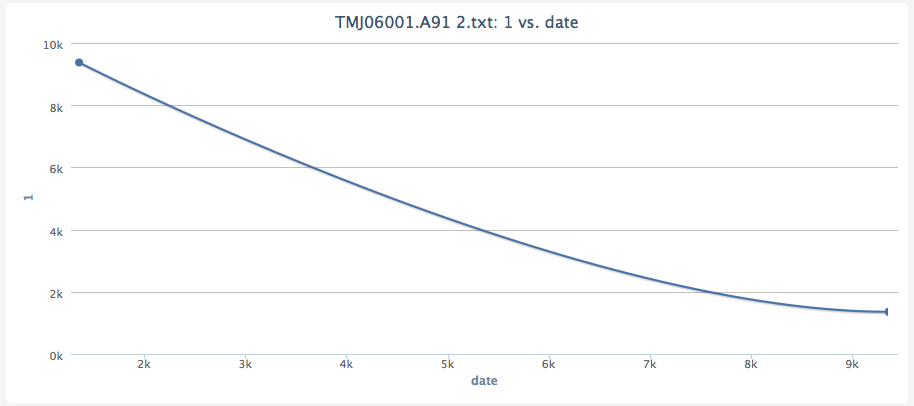
\includegraphics[width=120mm]{images/viz_ex1}
	\caption{A visualization example.} 
	\label{viz_ex1}
	\end{center}
\end{figure}

Hatch uses HighCharts, a JavaScript library, to perform visualizations. It
allows Hatch to incrementally stream new graph data to the client, instead of
resending all the graph data. This is useful when users are working on low
bandwidth connections, or with large datasets. By reducing unneeded data 
transfer, Hatch is able to work with larger datasets faster.

Hatch is able to check incrementally for new data. When data is graphed, it points towards the 
data in the document that needs visualization. If the data in the document changes,
the graph adds the data points to the graph without refreshing the page.

This opens up the possibility of Feeds. Feeds are scheduled events in Hatch that pull
JSON data from somewhere on the web. They push the data in to the document they point
to. This data can simultaneously be used by a visualization in order to immediately graph
the new data, as soon as a change is detected in the document.
The result is Live Charts, and documents that sync with data on the web when new data is 
available. Instead of doing a bulky request for data all at once, data can be taken
in smaller requests, and Hatch can give users a real-time view their data as it comes
into the system
